 %%%%%  Preamble  %%%%%
%\documentclass[12pt]{report}
%\input{/Users/dasirianni/Documents/tex_templates/article_preamble.tex}
\documentclass[aip,jcp,preprint,superscriptaddress,floatfix]{revtex4-1}
\usepackage{dcolumn}    % decimal align in tables
\usepackage{bm}                 % bold math
\usepackage{graphicx}        % Figures inside cells of tables
\usepackage{multirow}   % for table cells to span rows
\usepackage{pifont}     % for checkmarks
\usepackage{hyperref}  % for hyperlinks in doc
\usepackage{amsmath} % for writing mathematics and \align
\usepackage{amssymb}
\usepackage{rotating, booktabs}
\usepackage{longtable} % Multi-page tables
\usepackage[table]{xcolor} % Colored table cells
\usepackage[T1]{fontenc}
\usepackage{fancyvrb}
\usepackage{threeparttable}
\usepackage{makecell}
\usepackage[customcolors]{hf-tikz}
\usepackage{graphicx}
\usepackage{amssymb,amsmath,bm}
\usepackage{amsfonts} % Math fonts
\usepackage{amsthm} % Theorem handling
\usepackage{mathrsfs} % Math fonts
\usepackage{bbm} % For doublestruck 1
\usepackage{cancel} % Cancel terms to value in math mode
\usepackage{array} % Arrays
\usepackage{gensymb} % General symbols
\usepackage{pifont}     % for checkmarks
\usepackage{accents}
\usepackage{fancyvrb}
\usepackage{listings}
%\usepackage{minted}
%\usepackage{upquote}
%\usepackage{footnote}
%\definecolor{codegrey}{gray}{0.95}
%\usepackage[Q=yes]{examplep}

\usepackage{algorithm}
\usepackage{algpseudocode}
\VerbatimFootnotes
%\renewcommand*\listingscaption{Code Snippet}
%\renewcommand*\listoflistingscaption{List of Code Snippets}

\renewcommand{\sectionmark}[1]{\markleft{\thesection.\ #1}}
\renewcommand{\sectionmark}[1]{\markright{\thesection.\ #1}}
%\renewcommand{\chaptermark}[1]{\markboth{#1}{}}

\usepackage{titlesec}
\titleformat{\chapter}
  {\normalfont\LARGE\bfseries}{\thechapter}{1em}{}
\titlespacing*{\chapter}{0pt}{3.5ex plus 1ex minus .2ex}{2.3ex plus .2ex}

\setcounter{secnumdepth}{3}
\setcounter{tocdepth}{3}

\usepackage[titles]{tocloft}
\setlength{\cftsubsecnumwidth}{3em}
\setlength{\cftfignumwidth}{3em}
\setlength{\cfttabnumwidth}{3em}

% Additional Package Inclusion
\input{/Users/dasirianni/Gits/hiTeX/macros/mathematics}
%\input{/Users/dasirianni/Documents/tex_templates/thm_styles}

% Page Re-Formatting
\makeatletter
\renewcommand*{\thetable}{S-\arabic{table}}
\renewcommand*{\thefigure}{S-\arabic{figure}}
%\let\c@table\c@figure % Uncomment for shared table/figure numbering
\makeatother
\renewcommand{\thepage}{S-\arabic{page}}

%%%%%  Title, Author, & TOC  %%%%%
\begin{document}

\title{\textit{Supplementary Material to}\\
Variations on the Bergman Cyclization Theme: Electrocyclizations of Ionic
Penta-, Hepta-, and Octadiynes
}

\author{Dominic A. Sirianni}
\affiliation{Department of Natural Sciences, Daemen University, Amherst, NY
             14226}

\author{Xinli Song}
\affiliation{Department of Chemistry, University of Richmond, Richmond, VA
             23173}

\author{Salmika Wairegi}
\affiliation{Department of Chemistry, University of Richmond, Richmond, VA
             23173}

\author{Evan B. Wang}
\affiliation{Department of Chemistry, University of Richmond, Richmond, VA
             23173}

\author{Sebastian A. Mendoza-Gomez}
\affiliation{Department of Chemistry, University of Richmond, Richmond, VA
             23173}

\author{Adam Luxon}
\affiliation{Department of Chemistry, University of Richmond, Richmond, VA
             23173}

\author{Maxwell Zimmerly}
\affiliation{Department of Chemistry, University of Richmond, Richmond, VA
             23173}

\author{Ariana Nussdorf}
\affiliation{Department of Chemistry, University of Richmond, Richmond, VA
             23173}

\author{Michael Filatov-Gulak}
\affiliation{Department of Chemistry, Kyungpook National University, Daegu
702-701, South Korea}

\author{Roald Hoffmann}
\affiliation{Department of Chemistry, Cornell University, Ithaca, NY 14853}

\author{Carol A. Parish}
\email{cparish@richmond.edu}
\affiliation{Department of Chemistry, University of Richmond, Richmond, VA
             23173}

\date{\today}

\begin{abstract}
\vspace{2cm}
\textbf{Warning: Don't ever print this document --- it is long.}
\end{abstract}

\maketitle

%%%%%  BEGIN index content  %%%%%
\clearpage
\tableofcontents
\begingroup
\let\clearpage\relax
\listoffigures
%\addcontentsline{toc}{section}{\listfigurename}
\listoftables
%\addcontentsline{toc}{section}{\listtablename}
%\listofalgorithms
%\addcontentsline{toc}{section}{\listalgorithmname}
\endgroup
\clearpage

%%%%%  END index content  %%%%%

%%%%%  BEGIN Additional Materials Content  %%%%%

%\section{Additional Computational Details\label{ch:methods}}

\section{Theoretical Background\label{sec:theorybg}}

We are interested in characterizing Bergman-like electrocyclization reactions,
in which the reactants are closed-shell, ground state singlets and the products
are (presumably) aromatic diradicals.  Diradicals are theoretically challenging
molecules [10.1021/bk-2015-1209.ch011, 10.1021/acs.chemrev.9b00260] in which
two electrons occupy two quasi-degenerate orbitals, the electronic states of
which may be approximately described within the context of a two-level system,
visualized schematically in Fig.~\ref{fig:2level}.  For sufficiently small
orbital energy splitting, the resulting six electronic configurations
(Fig.~\ref{fig:2level}.a.i) combine to produce four symmetry-adapted electronic
states: two closed-shell, two-configurational singlets ($\Psi_+^{\rm TCS}$ and
$\Psi_-^{\rm TCS}$), one open-shell singlet ($\Psi^{\rm OSS}$), and three
degenerate components of the triplet ($\Psi_{M_s=-1}^{\rm T}$,
$\Psi_{M_s=0}^{\rm T}$, and $\Psi_{M_s=+1}^{\rm T}$), provided in
Fig.~\ref{fig:2level}.a.ii-iii.  Aside from the high-spin components of the
triplet ($\Psi_{M_s=\pm1}^{\rm T}$), each of these electronic states are
multiconfigurational, requiring more than one Slater determinant to adequately
describe the total wavefunction (referred to as static electron correlation).
While a compact, two-configurational self-consistent field (TCSCF) wavefunction
would be sufficient to capture the static correlation in this isolated
two-level system, real diradicals are not so simple: in addition to the
possibility of other quasidegenerate orbitals, whereby a more general,
multiconfigurational self-consistent field (MCSCF) wavefunction is required,
the contributions of instantaneous, pairwise electron-electron repulsion must
also be captured. This dynamical electron correlation necessitates the use of a
post-MCSCF, multireference approach, e.g., MR-PT, MR-CI, MR-CC, etc. in order
to adequately describe the properties and chemical behavior of these molecules.
Determining the reference active space (Fig.~\ref{fig:2level}.a.i) for
molecules such as these is complicated, and MR approaches
(Fig.~\ref{fig:2level}.a.ii-iii; e.g., MR-CC), are computationally intensive
for even small systems with only a few heavy (i.e., non-hydrogen) atoms.64, 67
Furthermore, if the transition states in these Bergman-like cyclizations are
product-like, they too may possess significant diradical character; due to the
additional complications inherent to transition-state searches, the application
of MR approaches to quantitatively examine diradical-producing reactions has
also been limited.

\begin{figure}[h!tp]
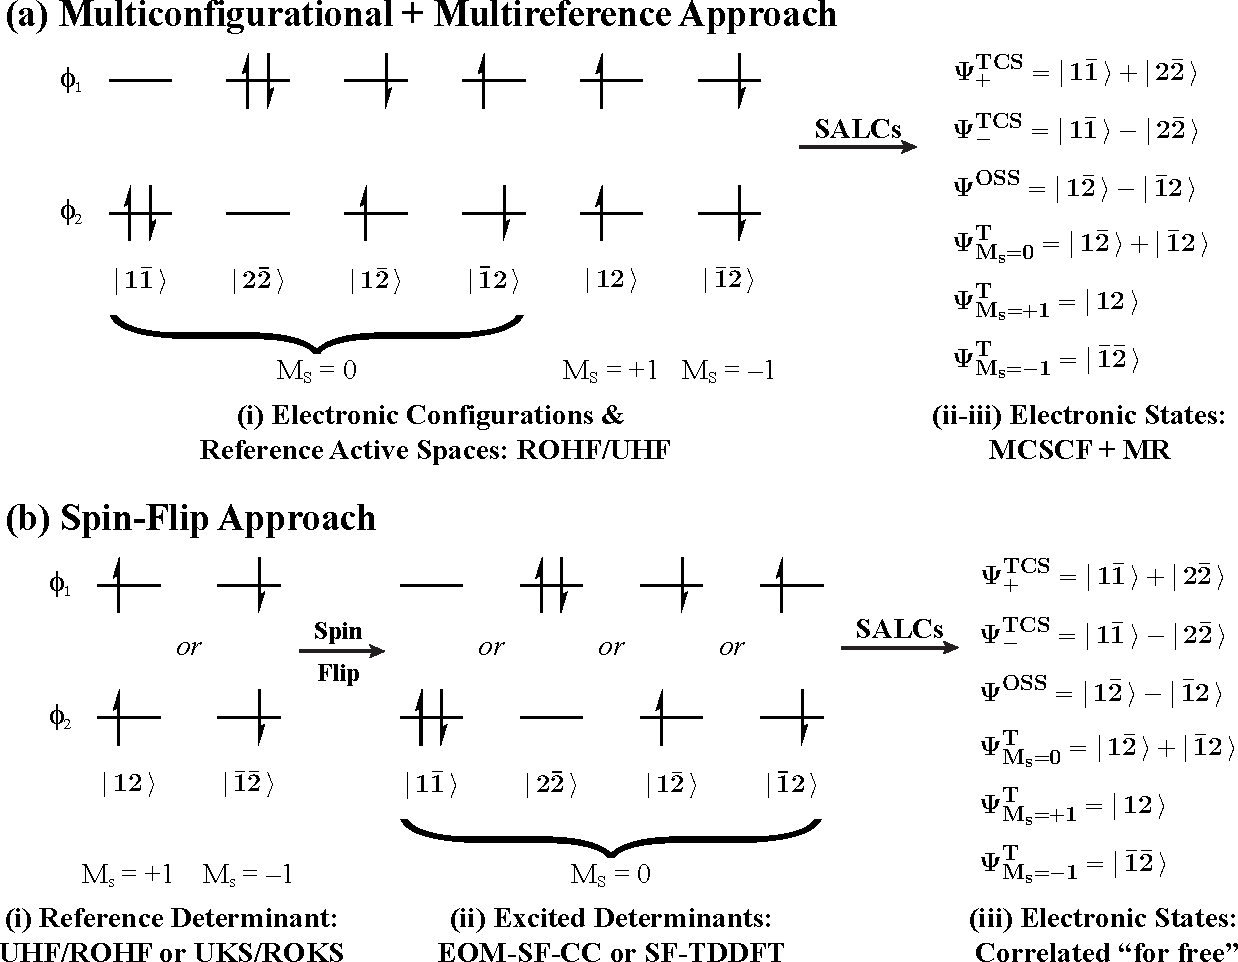
\includegraphics[width=\textwidth]{includes/MRvsSF-2level.pdf}
\caption[Quantum chemistry on two-level systems]{Schematic
representations of two different approaches to study diradical molecules,
within the context of a simple two-level system comprised of two electrons
(labeled 1 and 2) in two quasidegenerate orbitals $\phi_1$ and $\phi_2$.
Permutations of the orbital occupations in this two-level system produces six
distinct electronic configurations, represented above as a Slater determinant
$\ket{\phi_1(i)\phi_2(j)}\equiv\ket{ij}$ with electron $i$ occupying the
spatial orbital $\phi_1$ and electron $j$ occupying $\phi_2$ and where an
overbar denotes an electron has $\beta$ spin.}
\label{fig:2level}
\end{figure}

Alternatively, spin-flip (SF) formulations of excited state methods based on
single-reference theories like equation-of-motion coupled-cluster (SF-EOM-CC;
abbreviated SF-CC)51-58 or time-dependent density functional theory
(SF-TDDFT)49-50 have been developed that approach these systems in a different
way, visualized in Fig.~\ref{fig:2level}.b.  In the SF approach, a high-spin
($M_s = \pm1$) triplet reference is constructed with an open-shell
self-consistent field approach using either a restricted or unrestricted
reference (UHF/ROHF or UKS/ROKS; Fig.~\ref{fig:2level}.b.i), before spin-flip
excitations being performed to generate all low-spin ($M_S = 0$) excited
determinants (Fig.~\ref{fig:2level}.b.ii). These determinants may then be
combined and symmetry-adapted using the squares of the transition amplitudes
generating each spin-flipped determinant as expansion coefficients to generate
multiconfigurational states for which both static and dynamical electron
correlation is captured (Fig.~\ref{fig:2level}.b.iii).  In this manner, the
problem of applying a post-MCSCF multireference approach to capture both the
static and dynamical electron correlation in these systems is reduced within
the framework of a relatively more straightforward, computationally tractable
single-reference theory where dynamical electron correlation is included ``for
free'' (i.e., not requiring a subsequent correlated computation on top of the
spin-flip treatment generating the multiconfigurational states of interest).
Recently, computational investigations of the canonical Bergman cyclization
leveraging SF-TDDFT and SF-CCSD have exhibited good agreement with experimental
reaction barriers and thermodynamic quantities,17,49  the success of which
inspires us to apply these approaches in this work. 

\section{Development of Novel Characterization Approaches\label{sec:dev}}

\subsection{Linear Transit Approach for Transition-State Searching \&
Qualitative Reaction Profiling\label{subsec:lintransit}}

In the field of quantum chemistry, where most computational procedures are
notoriously ill-conditioned and difficult to perform, the geometric
optimization of transition state (TS) structures is among the least
well-behaved classes of computations that are still performed routinely.
Nevertheless, TS searching is a critical step in the quantitative
characterization of chemical reaction kinetics as well as the determination of
reaction  mechanisms, making them a necessary ingredient in studies such as
this work.  Like any geometry optimization, the goal of a TS search is to find
a stationary point on the nuclear potential energy surface (PES), where the PES
for a molecule comprised of N atoms is defined as a function of $3N-6$ mutually
orthogonal, internal degrees of freedom (or $3N-5$ for linear molecules)
mapping the molecular geometry to its potential energy.  In this context, a
stationary point on the PES is a molecular geometry for which the first
derivative of the electronic energy with respect to perturbation in nuclear
coordinates (the gradient) is zero.  

For conventional (i.e., non-TS) geometry optimizations, the end goal is to find
a stationary point which is also a minimum on the PES, where the curvature of
the surface --- defined as the sign of the second derivative with respect to
nuclear perturbation (the Hessian) at a particular set of nuclear coordinates
--- is positive when evaluated along all internal degrees of freedom.  The
procedure for finding such a point on the PES can be understood conceptually as
walking ``downhill'' from an initial guess structure: by first computing the
gradient vector at a given geometry and then perturbing the nuclear positions
to minimize the energy along that vector, a new structure can be generated
whose energy is lower than the previous one. Eventually, by iteratively
repeating this procedure to refine the initial structure, an optimal molecular
geometry can usually be found.  In practice, however, and especially in the
case of large molecules, the $3N-6$ internal degrees of freedom which define
the PES makes the brute-force search for an optimal molecular geometry either
prohibitively expensive or too ill-conditioned to be realistic. This makes the
choice of a ``good'' initial guess structure of paramount importance to ensure
successful completion of the optimization procedure.\cite{tschallenge}
Fortunately, chemical intuition and the use of classical potentials (force
fields) to refine an initial molecular structure can typically generate an
initial guess geometry lying close enough on the PES to the optimal one to be
able to seed a successful optimization.  

Unlike for conventional geometry optimizations, however, TS searches seek to
find a stationary point where the curvature is positive in all directions
except one; such stationary points are referred to as first-order saddle
points, thanks to their resemblance to an equestrian saddle.  Furthermore, the
specific direction in which the curvature of the PES is negative must
``connect'' the desired reactant(s) and product(s) structures, i.e., moving the
atoms in the direction of negative curvature will transform the reactant(s) to
the product(s). Clearly, TS searches are a much more complicated process than
simply walking downhill from an initial guess structure, making the choice of
an initial transition state structure all the more paramount.  Unfortunately,
arriving at good initial structures for TS searches is widely held to be more
of an art than a science, relying primarily on experience, chemical intuition,
and no small amount of luck.  During the course of this work, one of us (DAS)
ran out of ideas for generating different guess structures according to this
artful approach when faced with yet another unsuccessful TS search, leading to
the development of a more systematic, although less aesthetically pleasing,
approach for generating guess structures from which to begin TS searches, which
is described here. We include this discussion not as a scientific novelty ---
even though we are not aware of this approach being previously published in the
literature --- but as as a service to the community, with the hope of making TS
searches more approachable and routinely successful for practitioners in the
field.

As described above, the goal of a TS search is to find a saddle point on the
potential energy surface whose one degree of freedom with negative curvature
directly connects the reactant(s) and product(s).  Confirming the
identification of the desired TS therefore requires computing the vibrational
frequencies and normal modes of vibration at the identified stationary point;
this frequency analysis should reveal exactly one imaginary (may be represented
as negative) vibrational frequency, whose associated normal mode of vibration
traces a path of atomic displacement connecting reactant and product.  It would
be intuitive, then, to try to construct a pathway along this vibrational mode
to identify the transition state in a reduced search space (optimizing in only
one degree of freedom instead of 3N-6).  Indeed, this is exactly the goal of,
e.g., the frozen string\cite{x} and intrinsic reaction coordinate (IRC)\cite{x}
approaches, which have become major tools aiding in the identification of
transition states. These approaches do suffer from their own complexities and
numerical instabilities,\cite{x} however, and can therefore be difficult to
converge in their own right.  To avoid such issues while retaining the spirit
of these path-tracing methodologies, our approach connects reactant and product
species directly, with no normal mode information, by simply constructing a
geometric ``displacement vector'' from the difference in atomic positions between
the two structures.  We then scan the potential energy along this displacement
vector by incrementing the molecular structure of the reactant with respect to
the fractional extent of reaction, $\xi$ (where $\xi = 0$ corresponds to the
reactant and $\xi = 1$ to the product).  

Finally, transition state searches can
be seeded from these interpolated molecular geometries near the maximum of
energy computed along the profile.

\begin{figure}[ht!p]
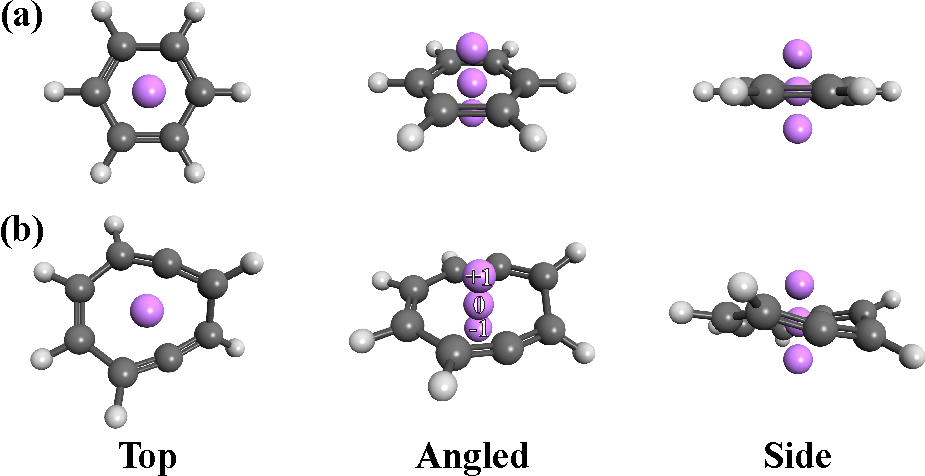
\includegraphics[width=\textwidth]{includes/nics-probes.pdf}
\caption[Novel scheme for uniquely placing NICS probes]{NICS(-1, 0, +1) probes
(lilac spheres) superimposed on structures for (a) benzene and (b) {\bf 8cTL}
as viewed from above (left panel), the side (right panel), or an angled
perspective (center panel).}
\label{fig:nics-probes}
\end{figure}

\subsection{Towards a General Approach for Placing NICS
Probes\label{subsec:nics-probes}}

As discussed in the Methods section of the main text, the standard location for
the placement of isotropic single-point NICS probes for planar, symmetric
aromatic molecules is in the center of the ring plane [for NICS(0)] and 1 \AA\
above and below the ring plane [for NICS($\pm$1)], all three of which must be
equidistant from all ring atoms. For the highly nonsymmetric and nonplanar
cyclic molecules examined here, however, there are two problems with this
convention, namely (i) there does not exist a point (or points) which are
mutually equidistant from all ring atoms and (ii) the notions of ``above'' and
``below'' are ill defined in the absence of a ring plane. While the first
concern is easily circumvented by taking inspiration from the literature 3
where the NICS(0) probe location was originally defined to coincide with the
non-mass--weighted geometric centroid of the ring, the second is still an open
question with several conventions existing in the literature for symmetric,
non-planar molecules.4  Rather than performing a much more involved and costly
analysis based on mapping the isotropic NICS values along a grid surrounding
our molecules, we have instead determined a system which is capable of
unambiguously placing these probes in a manner analogous to NICS($\pm$1) for
our nonsymmetric molecules that will recover previously reported conventions
when applied also to symmetric molecules.

To derive where the NICS($\pm$1) probes should be placed in the more general
case of a nonsymmetric, nonplanar molecule, it is intuitively sufficient to
begin by examining where these probes are placed for the conceptually simplest
aromatic molecule: benzene. In benzene, the NICS(0) probe is placed in the
center of the ring plane, with NICS($\pm$1) probes placed 1 \AA\ perfectly
above and below the molecular plane (see Fig.~\ref{fig:nics-probes}.a for
visualization). By connecting these points, it is clear that they lie on a line
which coincides with the principal axis of rotation (i.e., the $C_6$ axis of
the $D_{6h}$ point group). While not all molecules possess a principal rotation
axis defined by their symmetry, all molecules do possess a rotational reference
frame defined by the rotational moments of inertia as originally outlined in
the classic text by Wilson, Decius and Cross. 5 For symmetric molecules, the
principal axis of rotation (by symmetry) does coincide with one of the vectors
defining this rotational frame, namely the principal moment of inertia. These
moments of inertia are defined to be the eigenvectors of the moment of inertia
tensor, $\dunder{I}$, a $3\times3$ matrix with elements given by
\begin{align}
I_{\alpha\alpha} &= \sum_n\left(\beta_n^2 + \gamma_n^2\right)\\
I_{\alpha\beta} &= -\sum_n\alpha_n\beta_n
\end{align}
where $\alpha_n$, $\beta_n$, and $\gamma_n$ are mass-weighted Cartesian
coordinates for atom $n$, within which the origin of the coordinate frame is
defined to be the molecular center-of-mass.  The three moments of inertia which
define the rotational reference frame, $\left\{\ket{i_n}: n =
a,\,b,\,c\right\}$, are the eigenvectors which diagonalize the moment of
inertia tensor, $\dunder{I}$:
\begin{equation}
\dunder{I}\ket{i_n} = I_n\ket{i_n}
\end{equation}
It is worth noting that the eigenvalues $\left\{I_n: n = a,\,b,\,c\right\}$ are
related to the conventional (i.e., spectroscopic) rotational constants $N =
A,\, B,\, C$ according to
\begin{equation}
N = \frac{h}{8\pi^2 I_n}.
\end{equation}

To place the NICS(±1) probes for a general, non-symmetric and non-planar
molecule, we must take several additional considerations into account, namely 
\begin{enumerate}
\item the atoms being considered in the construction of the moment of inertia
tensor are only the ring atoms (i.e., the eight carbon atoms of 8cTL),
\item the origin of the coordinate system should be the non—mass-weighted
centroid of the ring atoms, rather than the center-of-mass, and
\item we are only interested in the principal moment of inertia, which
coincides with the principal symmetry axis for symmetric molecules.
\end{enumerate}
Therefore, we may simply diagonalize the non-mass--weighted moment of inertia
tensor $\dunder{\tilde{I}}$, constructed within the non-mass--weighted
coordinate frame defined by coordinates $\tilde{\alpha}$, $\tilde{\beta}$,
$\tilde{\gamma}$ and whose origin is placed at the ring centroid according to
the eigenequation
\begin{equation}
\dunder{\tilde{I}}\ket{\tilde{i}_n} = \tilde{I}_n\ket{\tilde{i}_n},
\end{equation}
at which point our NICS($\pm$1) probes may be placed 1 \AA\ in either direction
along the principal moment of inertia in this reference frame,
$\ket{\tilde{i}_a}$, as visualized in Fig.~\ref{fig:nics-probes}.b for species
{\bf 8cTL}. For the convenience of the reader and as a service to the
community, we have provided a script capable of automating this process written
in the highly readable Python programming language.  See
\url{https://github.com/Parish-Lab/Bergman-Variations-578} for instructions to
download, install, and use this script.

%%%%%  END Additional Materials Content  %%%%%

%%%%%  BEGIN Supplementary R&D  %%%%%

\section{Supplementary Results \& Discussion\label{sec:results}}

\subsection{Cyclization of the Penta-1,4-diyne Anion\label{subsec:5mem}}

\subsection{Absolute \& Relative Electronic Energies \& Enthalpies for All
Cyclizations\label{subsec:energy-tables}}

\subsection{Nucleus-Independent Chemical Shift Data\label{subsec:nics-data}}

\subsection{Qualitative Energetic Profiling of Cyclization Processes via Linear
Transits\label{subsec:lintransit-data}}

\subsection{Methodological Comparison: REKS vs.
EOM-SF-CCSD\label{subsec:reks-data}}

%%%%%  END Supplementary R&D  %%%%%

%%%%%  BEGIN bibliography  %%%%%

\clearpage
\newpage
\bibliography{/Users/dasirianni/Gits/hiTeX/bibtex/zotero,/Users/dasirianni/Gits/cdsgroup/papers/dsdb/jrncodes,/Users/dasirianni/Gits/cdsgroup/papers/dsdb/mainbib-ds,/Users/dasirianni/chem/parish-lab/projects/expanded-Bergman/manuscript/suppmat/latex/miscbib}

%%%%%  END bibliography  %%%%%

\end{document}

